%\section*{\lbtitle Определение дыхательного коэффициента прорастающих семян}
%\addcontentsline{toc}{section}{Определение дыхательного коэффициента прорастающих семян}

%\subsection*{Теоретические положения}

%\paragraph{}\efbox[margin=10pt,backgroundcolor=yellow]{
%	\begin{minipage}{0.95 \textwidth}
%	Дыхательный коэффициент (ДК) – это отношение количества $CO_2$, выделившегося в процессе дыхания, к поглощенному за это время кислороду ($CO{_2}/O{_2}$).
%	\end{minipage}
%	}	

%\paragraph{}Дыхательный коэффициент служит характеристикой калорийности субстрата и зависит от вида дыхательного субстрата и степени его окисленности. 

%\paragraph*{}В качестве субстрата для дыхания могут использоваться жиры, белки, углеводы и органические кислоты. Чем больше окислен материал, тем меньше поглощается кислорода воздуха, а значит и меньше выделяется энергии. Если в процессе дыхания используется углеводы, то ДК равен единице. Это следует из балансового уравнения окисления глюкозы \ref{glucosa_reaction}:

%\begin{equation}
%\label{glucosa_reaction}
%	C{_6}H_{12}O{_6} + 6O{_2} \rightarrow 6H{_2}O + 6CO{_2}
%\end{equation}
 

%\paragraph*{}В данном уравнении отношение $6CO{_2}/6O{_2}$ равно 1. При окислении жирных кислот и белков ДК будет меньше единицы так как они насыщены кислородом в меньшей степени, и, следовательно, на их окисление идет больше $O2$. Так, в случае окисления масляной кислоты \ref{oil_acide_reaction}:

%\begin{equation}
%\label{oil_acide_reaction}
%	CH{_3}-CH{_2}-CH{_2}-COOH + 5O{_2} \rightarrow 4H{_2}O + 4CO{_2} 
%\end{equation}

%ДК = $4CO{_2}/5O{_2}$ = 0,8

%\paragraph*{}При использовании в качестве субстрата дыхания более окисленных органических кислот, ДК будет больше единицы: 

%$C{_4}H{_4}O{_5} + 2,5O{_2} \rightarrow 2H{_2}O + 4CO{_2}$, 

%ДК =  $4CO{_2}/2,5O{2}$ = 1,6. 

\begin{footnotesize}

\paragraph*{}\textbf{Цель работы}: \hypertarget{breazing_index_lab}{Определить} \hyperlink{breazing_index}{\gls{breazingIndex}} прорастающих семян гороха;

\paragraph*{}\textbf{Оборудование}: Наклюнувшиеся семена гороха, пробирка с притертой пробкой, изогнутая под прямым углом стеклянная трубка, линейка, штатив
для пробирок, фильтровальная бумага, фарфоровые чашки, пинцеты, пипетки, часы;

\paragraph*{}\textbf{Реактивы}: 20-ный\% раствор КОН, окрашенная вода в
химическом стаканчике;

\end{footnotesize}

\subsection*{Ход работы}

\paragraph*{}Поместите в пробирку проклюнувшиеся семена гороха таким образом, чтобы пробирка была заполнена семенами примерно до половины. 

\paragraph*{}В изогнутую трубку поместите каплю окрашенной жидкости. Для этого опустите трубку в стакан с окрашенной жидкостью, после чего противоположный конец трубки закройте пальцем. Затем закройте пробирку с семенами пробкой с изогнутой трубкой.

\paragraph*{}Собранный и готовый к опыту прибор должен выглядеть следующим образом (\ris \ref{breazing_index}). 

%%%%%%%%%%%%%%%%%%%%%%%%%%%%%%%%%%%%%%%%%%%%%%%%%%%%%%%%%%%%%%%%%%%%%%%%%%%%%%%%%%%%%%%%%%%%%%%%%%%%%%%%%%% 
\begin{figure}[h!]
  \centering
       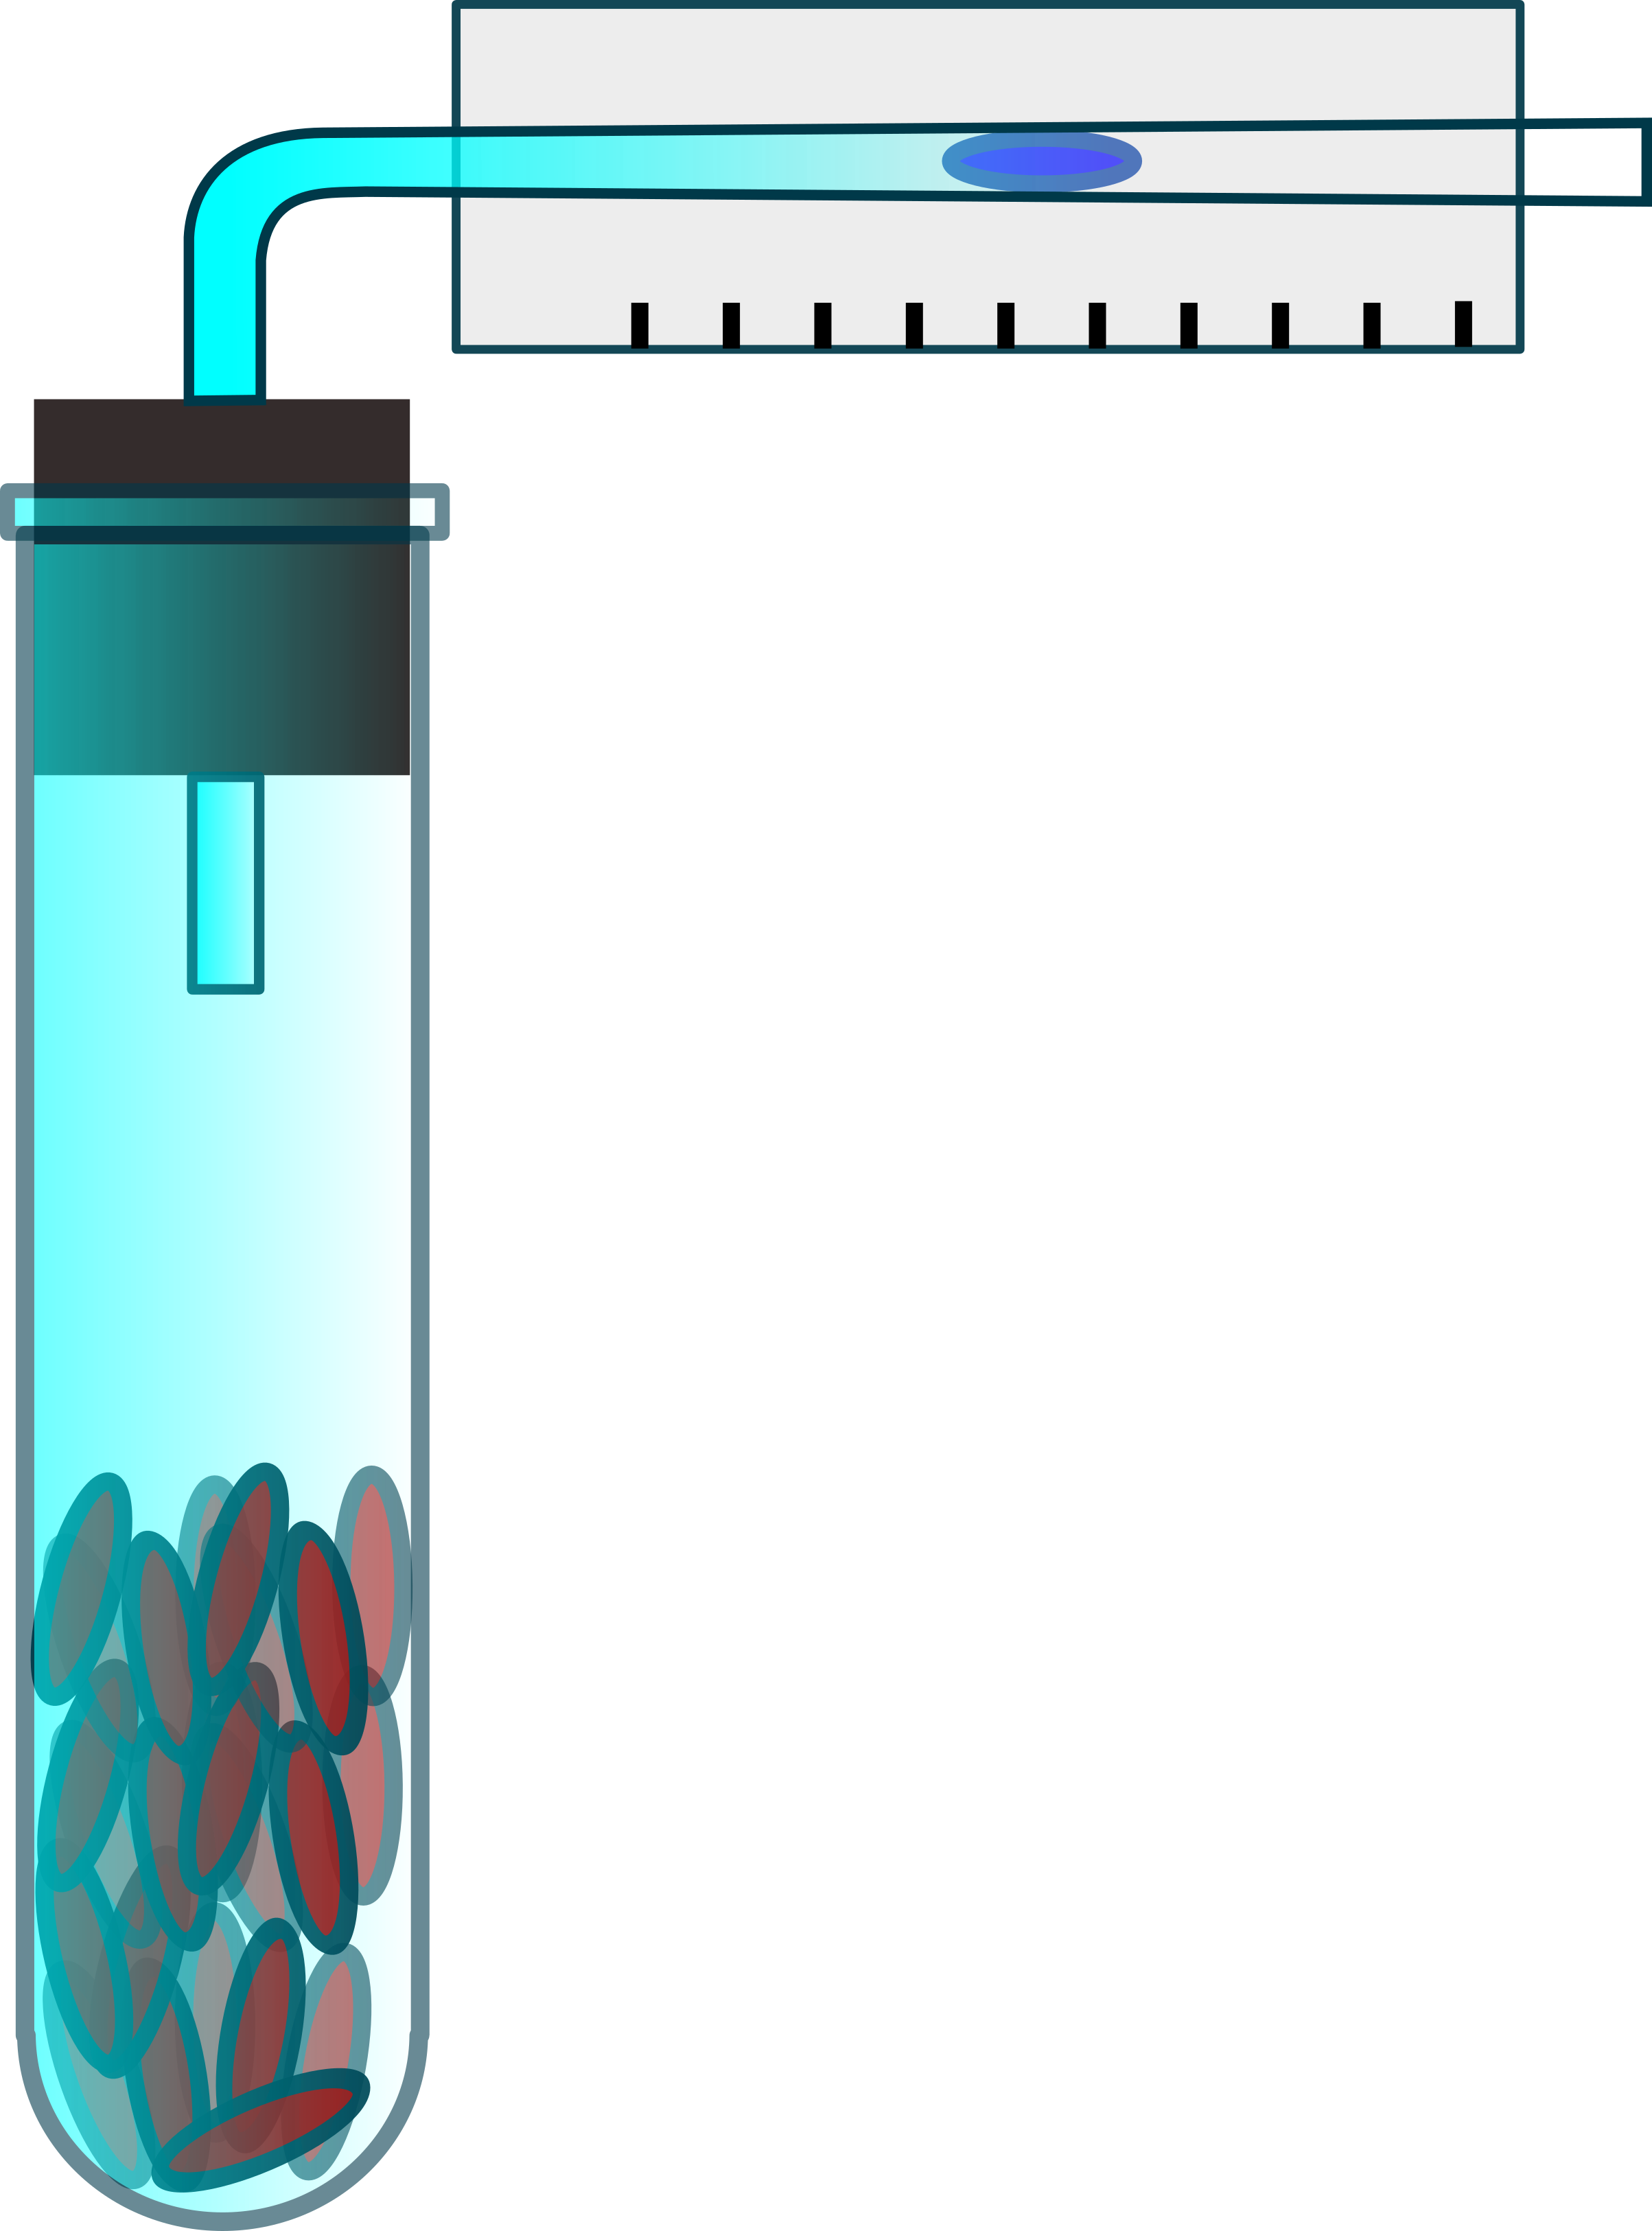
\includegraphics[width=0.3\linewidth]{pictures/breazing_index}
\caption{Прибор для измерения дыхательного коэффициента}
\label{breazing_index}
\end{figure}
%%%%%%%%%%%%%%%%%%%%%%%%%%%%%%%%%%%%%%%%%%%%%%%%%%%%%%%%%%%%%%%%%%%%%%%%%%%%%%%%%%%%%%%%%%%%%%%%%%%%%%%%%%%

\paragraph*{}Собранный таким образом прибор помещается в штатив. Положение мениска, образованного окрашенной жидкостью отмечается в начале опыта и затем через каждые 5 минут. Опыт продолжатся 15 минут.

\paragraph*{}На основании проделанных в результате опыта измерений, вычислите среднее расстояние, пройденное каплей за 5 минут (таблица \ref{table_breezing_seeds} А). Это расстояние соответствует разности между объемами поглощенного кислорода и выделенного углекислого газа.

\paragraph*{}По окончании первой серии измерений, в пробирку с семенами пинцетом поместите фильтровальная бумага, смоченная раствором NaOH. Снова закройте пробирку пробкой с изогнутой трубкой. Отметет положение мениска в начале опыта и затем в течении 15 минут через каждые 5 минут (таблица \ref{table_breezing_seeds} Б). Расстояние, пройденное окрашенной каплей в трубке, будет соответствовать количеству поглощенного кислорода, так как выделившийся в ходе дыхания  углекислый газ будет поглощаться раствором NaOH.

\paragraph*{}\gls{breazingIndex} вычисляется по формуле \ref{k_breaz}:

\begin{equation}
  \label{k_breaz}
  k = \frac{CO{_2}}{O{_2}} = \frac{(B - A)}{B}
\end{equation} 

\paragraph*{}Где \textit{А} - количество выделившегося углекислого газа, измеренное во время первого опыта, \textit{B} - количество поглощенного кислорода, измеренное во время второго опыта.

\paragraph*{}Результаты наблюдения запишите в таблицу \ref{table_breezing_seeds}.

\begin{table}
\centering
	\label{table_breezing_seeds}
	\caption{Форма заполнения результатов}
	\begin{tabularx}{\linewidth}{|p{5cm}|X|X|X|X|X|}
		\hline Условия & \multicolumn{4}{|c|}{Отсчет, мм 5 мин} & (В-А)/В \\ \cline{2-6}
		               &       1      &     2   &   3 & Среднее &         \\ 
		\hline Без щелочи (А)  &      &         &     &         &         \\
		\hline Со щелочью (Б)  &      &         &     &         &         \\
		\hline
	
	\end{tabularx}
\end{table}

\paragraph*{}На основе измерения дыхательного коэффициента, \textbf{сделайте вывод} о природе субстрата, служащего для дыхания прорастающих семян.

\subsection*{Вопросы для самоконтроля}

\begin{itemize}
	\item Какие факторы будут влиять на интенсивность дыхания?
	\item При каких условиях случается выпревание озимых? Каким образом гибель растений от выпревания связанна с дыханием?
	\item В чем заключается роль кофермента \gls{nadh} в процессе дыхания?
	\item В чем заключается сущность окислительного фосфорилирования?
	\item Какой процесс является общим как для брожения так и для аэробного дыхания? В чем сущность этого процесса?
	\item В чем заключается роль цикла Кребса для метаболизма растений?
\end{itemize}


%\chapter{Минеральное питание растения}

%\paragraph*{}Важнейшими \hypertarget{nutrition}{химическими} элементами, входящими в состав растения являются С, О, Н, N, Р, S. Среди этих элементов, углерод, кислород и водород поступают в организм растения из воздуха в виде воды и углекислого газ. В свою очередь Азот, фосфор, сера, а так же ряд других элементов, таких как калий, магний, железо, поступают из почвы через корневую систему в виде минеральных соединений.

%\paragraph*{}Все элементы в зависимости от их количественного содержания разделяются на макроэлементы (> 0,01\%) – N, Р, S, К, Са, Mg, Fe и микроэлементы (< 0,01\%) – Mn, Сu, Zn, В, Mo, О.

%\paragraph*{}Потребность растений в различных минеральных элементах может быть охарактеризована правилами, сформулированными  Ю. Либихом:

%\begin{itemize}
%	\item все элементы равнозначны и полное исключение любого из них приводит растение к гибели;
%	\item ни один из элементов не может быть заменён другим, даже близким по химическим свойствам, т. е. каждый элемент имеет своё специфическое физиологическое значение и по этой причине продуктивность культурных растений, в первую очередь, зависит от того питательного вещества (минерального элемента), который представлен в почве наиболее слабо. Данный закон получил название \textit{закона минимума Либиха}\cite{berezina_2009}. 
%\end{itemize}

%\paragraph*{}Таким образом, каждый из химических элементов, входящих в состав растения играет свою важную роль в метаболизме. Например такие элементы как C, O, H образуют структуру органических молекул, K, Na присутствуют в виде ионов участвуя в процессах регуляции метаболизма, Mn, Сu, Fe входят в состав активных центров ряда важных ферментов.
